%=============================================================================
% Private and public returns to Enhanced Rock Weathering in Sub-Saharan Africa
% Draft manuscript for Agricultural Economics.
% Compiles with pdfLaTeX + bibtex on Overleaf (standard article class).
% Coauthors: switch to the Wiley/AgEcon class at submission if desired.
%=============================================================================
\documentclass[12pt]{article}

\usepackage[margin=1in]{geometry}
\usepackage{amsmath,amssymb}
\usepackage{graphicx}
\graphicspath{{figures/}}
\usepackage{booktabs}
\usepackage{caption}
\usepackage{subcaption}
\usepackage{setspace}
\usepackage[round]{natbib}
\usepackage{lineno}
\usepackage[colorlinks=true,allcolors=blue]{hyperref}
\usepackage{xcolor}

\newcommand{\todo}[1]{\textcolor{red}{[#1]}}
\newcommand{\tco}{\,t\,CO\textsubscript{2}}
\newcommand{\co}{CO\textsubscript{2}}

\doublespacing
\linenumbers

\title{\textbf{Mapping the potential public and private returns to
Enhanced Rock Weathering in Sub-Saharan Africa}}

\author{
  Bisrat Haile Gebrekidan\thanks{CIMMYT--Ethiopia. Corresponding author: \texttt{b.gebrekidan@cgiar.org}.} \and
  Jordan Chamberlin\thanks{CIMMYT--Kenya. \texttt{j.chamberlin@cgiar.org}.} \and
  \todo{Author Three}\thanks{Affiliation to be added (enhanced-weathering processes).}
}
\date{Draft: \today}

\begin{document}
\maketitle

\begin{abstract}
\noindent
Enhanced Rock Weathering (ERW) -- spreading finely ground silicate rock such as
basalt on cropland -- sits at an unusual intersection of two value streams: it
durably removes atmospheric \co{} (a public good, monetizable through voluntary
carbon markets, VCM) and it neutralizes soil acidity much like agricultural
lime, raising yields (a private return to the farmer). We develop a spatially
explicit, decomposed \emph{ex ante} profitability model for 44 Sub-Saharan African
(SSA) countries and 23 crops that separates the per-hectare gross margin of
basalt-ERW into an agronomic (private) term and a carbon (public) term, each
net of the full delivered cost. We map three decision-relevant envelopes: land
where the private return alone justifies investment, land where the public
return alone justifies it, and their intersection. Crediting only durably exported carbon -- deducting the alkalinity consumed
neutralizing soil acidity, which re-releases its \co{} just as lime does -- we
evaluate the public (carbon) and private (yield) cases together in the
equilibrium steady state. Under a spatially targeted lime-equivalent dose the
private envelope (4.3~Mha) exceeds the durable public envelope (1.7~Mha), and the
two coincide on 1.2~Mha; but the \emph{combined} envelope is far larger
(6.9~Mha), because on roughly 2.1~Mha neither stream alone covers the cost yet
together they do. This is the central economic result: voluntary carbon finance
is not a bonus on an already-profitable practice but the margin that makes an
otherwise-unprofitable agronomic investment viable. Properly accounting for
acidity neutralization cuts credited removal by about 80\% at first application
and shows that durable removal is largely a steady-state phenomenon; the carbon
case is bound by the realized \co{} removed per tonne of rock (median marginal
abatement cost \$446/\tco{}), the largest and least-resolved lever. We map a
robust core-targeting geography and the field-data priorities that would most
improve it.
\\[4pt]
\textbf{Keywords:} enhanced rock weathering; carbon dioxide removal; voluntary
carbon markets; soil acidity; agricultural liming; Sub-Saharan Africa;
additionality; \emph{ex ante} analysis. \\
\textbf{JEL:} Q12, Q15, Q54, Q56, O13.
\end{abstract}

%=============================================================================
\section{Introduction}\label{sec:intro}
% Structured on Head's formula: hook, question, antecedents, value-added, roadmap.

Enhanced rock weathering (ERW) has attracted considerable attention as a carbon
dioxide removal (CDR) pathway that promises climate mitigation while
potentially delivering material benefits to farmers
\citep{beerling2020,beerling2025nree}. The mechanism is well understood.
Silicate rock -- most commonly basalt -- is quarried, ground to a fine dust, and
spread on agricultural fields. There, rainwater and the \co{} respired by roots
and soil microbes form carbonic acid, which dissolves the silicate minerals;
this reaction consumes \co{} and converts it into dissolved bicarbonate
($\mathrm{HCO_3^-}$) while releasing base cations such as $\mathrm{Ca^{2+}}$ and
$\mathrm{Mg^{2+}}$. The bicarbonate is carried by drainage water through rivers
to the ocean, where the captured carbon is stored on geological timescales (in
excess of 10{,}000 years) \citep{beerling2020,renforth2019}. The same reaction
that sequesters carbon also neutralizes soil acidity: the released cations raise
soil pH and base saturation, relieving the aluminum and manganese toxicity and
nutrient-availability constraints that depress yields on acid soils, so that ERW
can raise crop yields much as agricultural lime does \citep{kantola2017,skov2024}.

While the mechanisms are well established, how ERW would play out in
practice -- particularly in data-limited geographies -- is far less
substantiated. In particular, the economics that underlie return-on-investment
calculations have not been evaluated in a spatially explicit, granular way,
which makes it difficult to know how and where to invest. This gap matters
because the public investment case, tied to carbon removal, may be spatially
distinct from the private case -- the locations where the value of yield gains
exceeds the cost of applying ERW. Where these two return surfaces diverge,
alternative funding strategies -- voluntary carbon market (VCM) financing,
private input-market development, or some blend of the two -- face very different
spatial opportunity sets. The absence of explicit, comparable estimates is thus
a barrier to investment and targeting. One concrete version of the targeting
problem is the question a carbon-market investor would ask: where can payments
for carbon sequestration also deliver benefits to smallholder farmers?

In this paper we take a spatially explicit, \emph{ex ante} modeling approach to
characterize the benefit streams that ERW would generate across different
geographical contexts in Sub-Saharan Africa (SSA), an understudied region with
large potential payoffs to the practice. Our approach is grounded in the
observation that the economics of ERW are fundamentally governed by spatial
conditioners: CDR potential depends on soil chemistry and rainfall; the yield
dividend from acidity neutralization varies with crop, soil type, and baseline
acidity; and the delivered cost of feedstock to the farm gate is built up from
quarry proximity, grinding energy, and transport distance. Bringing these
spatially varying factors into a single accounting framework, we evaluate how
the distributions of public and private returns compare with one another and
with the site-specific delivered cost of ERW.

Our work draws on and connects two largely separate literatures, reviewed in
Section~\ref{sec:lit}: a fast-growing body that substantiates the geochemistry
and carbon-removal potential of ERW but rarely examines its on-farm economics,
and a spatially explicit agronomic and economic literature on the returns to
soil-acidity remediation through liming. The few ERW yield trials in Sub-Saharan
Africa report responses in relative terms over short horizons, without economic
returns \citep{oppongdanso2025,akortey2026}, while the liming literature
\citep{vascosilva2025,hijbeek2021} supplies the integrated, spatially explicit
framework we adapt.

Our value-added is to take that liming framework and reconfigure it for ERW,
accounting jointly for the agronomic yield benefit and the carbon-removal
benefit, net of the spatially varying delivered cost of feedstock, while
operationalizing the mechanistic CDR understandings from the geochemical
literature at high spatial resolution. To our knowledge this is the first
analysis to map the private and public benefit streams of ERW side by side and
net of location-specific delivery costs. Doing so lets us delineate the
opportunity space for carbon-market financing, which is especially attractive
where it also delivers smallholder co-benefits, and ask where the private return
alone is large enough that a market for ERW could be built on farmers' own
willingness to pay.

We address six questions, the first three scoping the financing opportunity and
the last three turning the estimates into decisions and a model-improvement
agenda.
\begin{enumerate}
\item Where is there a case for a \emph{private market} for ERW, regardless of
  public returns -- that is, where do yield-based returns alone exceed the
  delivered cost, so that farmers or input suppliers could fund deployment
  without carbon finance?
\item Where is there a case for \emph{voluntary-carbon-market (VCM) investment},
  regardless of private returns -- where does the value of durable carbon removal
  alone exceed the delivered cost?
\item Where do the two \emph{coincide}, strengthening the proposition for a carbon
  buyer -- where a purchased tonne of removal also delivers a smallholder yield
  co-benefit?
\item How robust are these answers to parameter uncertainty (delivered cost,
  carbon price, yield response, CDR rate, and the carbon-accounting choice)?
\item Given that uncertainty, which areas should early \emph{pilots} target?
\item Which assumptions and processes -- and in which areas -- would targeted
  \emph{field data} most improve, to drive an iterative modeling loop?
\end{enumerate}
A point on framing: the private return and the carbon-market \emph{co-benefit}
are the same quantity -- the economic value of ERW-induced yield gains -- seen from
two vantage points, the smallholder who captures it directly and the carbon buyer
who values it as bundled impact. Questions~1--3 map onto the private, public, and
intersection return surfaces we estimate.

The remainder of the paper is organized as follows.
Section~\ref{sec:lit} reviews the relevant literature in more detail.
Section~\ref{sec:methods} sets out our conceptual framework and modeling
approach. Section~\ref{sec:results} presents our core results and the
sensitivity of our conclusions to parameter uncertainty.
Section~\ref{sec:discuss} discusses how the results may inform investment
strategies, pilot-program targeting, and further research, and
Section~\ref{sec:conclude} offers concluding remarks.

%=============================================================================
\section{Background and related literature}\label{sec:lit}
\paragraph{ERW as a joint product.}
Enhanced rock weathering is distinctive among carbon-removal options in producing
two benefits from a single action. When crushed silicate rock, typically basalt,
dissolves in soil, the reaction consumes carbonic acid and converts \co{} into
bicarbonate while releasing base cations such as $\mathrm{Ca^{2+}}$ and
$\mathrm{Mg^{2+}}$ \citep{beerling2020,kantola2017}. The bicarbonate, once it
leaches to rivers and the ocean, stores carbon on geological timescales; the same
cations raise soil pH and relieve the aluminum and manganese toxicity that
depress yields on acid soils, so the agronomic effect closely parallels
agricultural lime \citep{lewis2021}. The contrast with lime is instructive, since
lime's alkalinity carries carbon that is re-released when it neutralizes acidity,
making liming carbon-neutral at best, whereas the silicate's alkalinity is
generated by consuming atmospheric \co{}. Field trials increasingly document the
yield side of this joint product, in temperate systems \citep{skov2024} and, in
Sub-Saharan Africa, in Ghanaian maize amended with fine-grained silicate rock
flour \citep{oppongdanso2025,akortey2026}. It is this coupling of a public good
and a private good in one practice that motivates analyzing the two returns
together.

\paragraph{CDR potential and cost.}
A large literature estimates the carbon-removal potential and cost of ERW. Early
techno-economic work derived global potentials and \$/\tco{} cost curves and
identified grinding energy and feedstock chemistry as the dominant cost and
efficiency levers \citep{strefler2018}, and continental assessments place
croplands at the center of feasible deployment \citep{beerling2020,beerling2025}.
Subsequent modeling has sharpened how climate governs weathering rates and hence
the spatial distribution of potential \citep{baek2023,deng2023}. A parallel and
still unsettled strand concerns how much of the gross weathering signal is
durable: bicarbonate can re-precipitate as pedogenic carbonate or fail to export,
so realized removal can fall well below stoichiometric ceilings
\citep{renforth2019,kanzaki2023}, and recent reviews stress the resulting
quantification and permanence uncertainties and the monitoring needed to resolve
them \citep{schiedung2026,levy2024,beerling2025nree}. This body of work is rich on
the geochemistry but typically frames ERW as a carbon supply curve, abstracting
from the farm economy in which deployment must actually occur.

\paragraph{Application rates in comparable assessments.}
Spatially explicit assessments of ERW on croplands have almost universally
applied a \emph{uniform} basalt rate, and those rates cluster in a narrow band
(Table~\ref{tab:rates}). Global and regional models use 10 to 50 t/ha, often
annually: 10 t/ha/yr in \citet{baek2023} and \citet{tu2026}, 40 t/ha/yr in
\citet{beerling2020} and \citet{beerling2025}, and 50 t/ha in the life-cycle and
techno-economic assessment of \citet{kroeger2026}. Field trials test a wider
range, from 10 to 20 t/ha in temperate \citep{skov2024} and West African
\citep{oppongdanso2025} experiments to 50 to 100 t/ha \citep{akortey2026}, and
on-farm smallholder deployments in India apply 25 to 50 t/ha with documented
yield and income gains \citep{jordan2026}; reviews note experimental rates as
high as several hundred t/ha \citep{schiedung2026}. Our uniform scenarios
(10/20/50 t/ha) therefore span the modeling mainstream, with our maximum at its
upper edge and well below extreme experimental doses. Our targeted allocation
departs from this literature: instead of a fixed uniform rate, it sizes the dose
to each soil's lime requirement, which is precisely what couples the carbon and
agronomic accounts and motivates the net-export correction of
Section~\ref{sec:netexport}.

\begin{table}[t]
\centering
\caption{Basalt application rates in comparable ERW assessments.}
\label{tab:rates}
\small
\begin{tabular}{l l p{3.7cm}}
\toprule
Study & Scope & Application rate \\
\midrule
\citet{baek2023}        & Global croplands (model)        & 10 t/ha/yr \\
\citet{tu2026}          & Global adoption/equity (model)  & 10 t/ha \\
\citet{beerling2020}    & Global croplands (model)        & 40 t/ha/yr \\
\citet{beerling2025}    & US croplands (model)            & 40 t/ha/yr \\
\citet{kroeger2026}     & Life-cycle / techno-economic    & 50 t/ha \\
\citet{skov2024}        & Temperate field trial (oat)     & 20 (up to 100) t/ha \\
\citet{oppongdanso2025} & Ghana field trial (maize)       & 10, 50 t/ha \\
\citet{akortey2026}     & Ghana field trial (maize)       & 50, 100 t/ha \\
\citet{jordan2026}      & India on-farm (rice)            & 25--50 t/ha \\
\midrule
This study              & SSA, spatial (private + public) & targeted (lime req.) + uniform 10/20/50 t/ha \\
\bottomrule
\end{tabular}
\end{table}

\paragraph{Soil acidity and the economics of liming in SSA.}
Because ERW is, agronomically, ``liming with a different rock,'' the
soil-acidity-remediation literature provides our closest methodological template.
Acid soils are widespread across SSA and impose large, quantifiable yield
penalties; recent continental work estimates that acidity depresses yields on
32.7~Mha, about 23\% of cropland, a roughly US\$6~billion burden, a substantial
share of which could be profitably alleviated by liming on the order of 6 to
9~Mha \citep{vascosilva2025}. That assessment builds on spatially explicit
lime-requirement models \citep{aramburumerlos2023} and connects to farm-level
analyses of the multi-year economics and greenhouse-gas trade-offs of liming, for
example in western Kenya \citep{hijbeek2021}. We adapt this integrated, spatially
explicit framework, reconfiguring its costs and crop-response functions for
basalt and adding the carbon-removal benefit and the delivered-cost geography that
ERW introduces.

\paragraph{Adoption and smallholder finance.}
Whether any of this potential is realized depends on who can finance it. The
defining feature of the ERW investment, as with liming, is a large upfront outlay
(on the order of \$600/ha for basalt) against benefits that accrue over several
seasons. For credit-constrained smallholders with short decision horizons, such
front-loaded investments are precisely those that the technology-adoption
literature identifies as systematically under-adopted absent finance, insurance,
or subsidy \citep{jack2013market}. This makes the locus of returns a first-order
question: where farmers themselves capture enough value to pay, deployment can
proceed through input markets or cost-sharing arrangements; where they do not, it
requires external finance. Estimating the private return is therefore not only of
academic interest but directly informs which financing instrument is feasible
where.

\paragraph{Voluntary carbon markets and additionality.}
The most discussed external financing channel for ERW is the voluntary carbon
market, where buyers increasingly favor removals that are durable, well
quantified, and accompanied by development co-benefits. Two considerations bear
directly on our analysis. First, integrity and measurement: because durable
removal is uncertain and partly offset by soil processes, conservative net
accounting matters for what can credibly be sold \citep{schiedung2026,levy2024}.
Second, additionality: a credit is meant to fund removal that would not otherwise
occur. Coupled private and public returns complicate this test in an informative
way. Where yield returns alone already justify the practice, carbon credits are
weakly additional; where neither return alone suffices but their sum does, carbon
finance is pivotal and clearly additional. The spatial structure of the two
returns is thus not incidental to crediting but central to it.

\paragraph{What is missing.}
Despite rich literatures on ERW geochemistry, on the economics of liming, and on
carbon-market design, no prior work, to our knowledge, estimates the spatial
distributions of the private (yield) and public (carbon) returns to ERW side by
side, characterizes where each is sufficient on its own and where only their
combination is, or frames the carbon credit as the marginal financing that
converts an otherwise-unprofitable yield-improving practice into a viable one,
particularly in a high-acidity, smallholder-dominated setting like SSA. Nor has
the durable-removal accounting that this coupling demands, in which alkalinity
consumed neutralizing soil acidity is not credited as exported carbon, been
applied spatially. We address these gaps.

%=============================================================================
\section{Conceptual framework and modeling approach}\label{sec:methods}
% -- FULL PROSE ---------------------------------------------------------------
\subsection{Private and public returns}\label{sec:concept}
Consider a representative cropland pixel and a one-off decision to apply crushed
basalt at an agronomically calibrated rate. The per-hectare gross margin of the
practice has three economic components: an agronomic return from the yield
response to acidity neutralization, $R_a$; a carbon return from selling the
verified \co{} removed, $R_c$; and the delivered cost of the basalt, $C$
(quarrying, grinding, transport, and spreading). All three are spatially
heterogeneous. We write the combined gross margin as
\begin{equation}
  \mathrm{GM} \;=\; R_a \;+\; R_c \;-\; C,
  \qquad R_c \;=\; \rho \,(p - m),
  \label{eq:gm}
\end{equation}
where $\rho$ is the net \co{} removed per hectare (t\,CO\textsubscript{2}/ha,
after life-cycle emissions, pedogenic-carbonate loss, and the alkalinity
consumed neutralizing soil acidity; Section~\ref{sec:netexport}), $p$ is the carbon
price (\$/\tco{}), and $m$ is the per-tonne MRV cost.

The novelty is not the combined margin but its \emph{decomposition} into a
private and a public test, each charged the \emph{full} cost of the practice:
\begin{align}
  \text{Private-sufficient:}\quad & \mathrm{GM}_a \equiv R_a - C > 0, \label{eq:priv}\\
  \text{Public-sufficient:}\quad  & \mathrm{GM}_c \equiv R_c - C > 0. \label{eq:pub}
\end{align}
Equation~\eqref{eq:priv} identifies land where a farmer would rationally invest
on yield grounds alone, ignoring carbon; equation~\eqref{eq:pub} identifies land
where a carbon buyer would fund the practice on removal grounds alone, ignoring
yield. Their \emph{intersection} ($\mathrm{GM}_a>0 \wedge \mathrm{GM}_c>0$) is
land where the investment is doubly justified -- and, crucially, where the carbon
credit is \emph{least additional}, because the agronomic case already stands on
its own. This yields a five-way typology of cropland
(Figure~\ref{fig:typology}): both, private-only, public-only,
\emph{combined-only} (neither stream alone covers $C$ but together they do,
$\mathrm{GM}>0$), and neither. The combined-only set is where carbon finance is
pivotal: it is additional by construction and it is precisely the land that VCM
revenue moves from unprofitable to profitable.

\paragraph{The public envelope is a marginal-abatement-cost test.}
Substituting $R_c=\rho(p-m)$ into \eqref{eq:pub} and noting that the per-hectare
application rate cancels between $\rho$ and $C$ (both scale linearly with tonnes
of rock applied), public-sufficiency reduces to
\begin{equation}
  \underbrace{\frac{c_t}{\delta_t}}_{\text{MAC}} \;<\; p - m,
  \label{eq:mac}
\end{equation}
where $c_t$ is the delivered cost per tonne of basalt and $\delta_t$ is the
\co{} removed per tonne of basalt. The public envelope is therefore exactly the
land whose marginal abatement cost (MAC) lies below the net carbon price. Because
$\delta_t$ -- the realized removal per tonne of rock -- is small and uncertain,
equation~\eqref{eq:mac} makes clear that the carbon case is governed first by the
\emph{CDR rate}, and only second by the credit price. This is the analytical
core of the paper's main empirical result (Section~\ref{sec:public}).

%=============================================================================
\subsection{Data and raster modeling framework}
We build on a per-pixel (\(\sim\)0.083\textdegree, \(\sim\)9~km) \emph{ex ante} model
covering 44 SSA countries and 23 SPAM crops. Soil properties (pH, exchangeable
acidity and bases, bulk density) come from SoilGrids \citep{poggio2021};
harvested area, production, and yield from SPAM \citep{yu2020}; climate from
WorldClim \citep{fick2017}; basalt source lithology from GLiM
\citep{hartmann2012}; a motorized friction surface for haulage cost-distance
from \citet{weiss2018}; and producer prices from FAOSTAT \citep{faostat}
(2016--2020 medians). Lime-equivalent requirements use the LiTAS method
\citep{aramburumerlos2023}; the agronomic suitability response uses EcoCrop.
Full layer provenance and constants are documented in the model repository.

\subsection{Cost, carbon, and agronomic terms}
Delivered cost per tonne of basalt is the sum of a quarry-gate price
(\$10/t), grinding (energy use $\times$ country electricity tariff), spatial
transport (travel-time $\times$ haulage rate), and spreading (\$8/t). Net \co{}
removal per tonne combines feedstock stoichiometry, a Lewis-calibrated reactive
fraction, a grain-size factor, a climate (temperature--moisture--pH) scalar, and
a deduction for alkalinity that re-precipitates locally as pedogenic carbonate;
it is then netted of grinding, transport, and spreading life-cycle emissions. The
agronomic return is the modeled yield response to acidity neutralization valued
at crop-specific producer prices. We adopt baseline parameters of a \$150/\tco{}
credit price, \$20/\tco{} MRV cost, 50~$\mu$m grain size, and a
10\% discount rate.

\subsection{Net-export carbon accounting}\label{sec:netexport}
The alkalinity released by weathering can either neutralize soil acidity or
export as bicarbonate to the ocean; it cannot do both. Alkalinity that
neutralizes exchangeable acidity re-releases the captured \co{}
($\mathrm{HCO_3^- + H^+ \to H_2O + CO_2}$, with protons supplied by
$\mathrm{Al^{3+}}$ hydrolysis), exactly as agricultural lime does -- which is why
lime is not a carbon-removal technology. Durable removal is therefore only the
alkalinity that exports \emph{beyond} the soil's acidity demand. We credit
\begin{equation}
  \rho_{\text{net}} \;=\; \max\!\big(\rho_{\text{gross}} - F\,S,\; 0\big),
  \label{eq:netexport}
\end{equation}
where $S$ is the soil's exchangeable acidity expressed as a lime requirement
(t\,CaCO\textsubscript{3}/ha, from the LiTAS/Kamprath calculation already in the
pipeline) and $F = 0.88$ t\,CO\textsubscript{2} per t\,CaCO\textsubscript{3}-eq
is the \co{} re-released per unit of acidity neutralized -- fixed by the
feedstock's own stoichiometry, not tuned. The sink is regime-specific: the
\emph{standing} exchangeable acidity at first application, but only the annual
\emph{re-acidification} in steady state. Equation~\eqref{eq:netexport} is a
first-order (sequential) bound: it assumes the acidity sink is filled before any
alkalinity exports, whereas in reality weathering, neutralization and leaching
occur together, so the truth lies between $\rho_{\text{net}}$ and
$\rho_{\text{gross}}$; we report both. A direct corollary, central to the
results, is that the agronomically optimal (lime-requirement) dose is
CDR-minimal: durable removal requires applying \emph{beyond} the acidity demand,
so the private and public objectives pull the application rate in opposite
directions.

\subsection{Over-liming penalty}\label{sec:overlime}
The same surplus alkalinity that exports as durable carbon also raises soil pH.
Where a dose pushes pH past a crop's optimum, yield declines through micronutrient
lockout and phosphorus retrogradation. Our baseline credits the yield response to
acidity relief but does not penalize this overshoot; as a refinement we evaluate
each crop's pH suitability at the \emph{post-application} pH. We estimate that pH
from the reacted alkalinity (equal to $\rho_{\text{gross}}$ on the same $F$ basis),
which first neutralizes the soil's exchangeable acidity and, once that demand is
met, raises pH into the alkaline range buffered by the soil's ECEC; a crop-specific
EcoCrop pH ceiling then haircuts the agronomic return above the crop's optimum.
This is a first-order refinement whose magnitude depends on the soil buffer
constant and the realized reactive fraction, which we carry as a sensitivity band
(Section~\ref{sec:durable}).

\subsection{Temporal regimes and allocation rules}
We report three temporal accountings: \emph{year-1} (undiscounted, agronomic
return summed over the 5-year basalt residency), \emph{NPV} at 10\% (carbon
revenue phased over five years and discounted; agronomic NPV over the
reapplication interval), and \emph{equilibrium} (steady-state maintenance dose).
Because durable carbon removal is intrinsically a steady-state quantity
(Section~\ref{sec:netexport}), we lead both the public and the private case on
the \emph{equilibrium} regime -- which places the two return streams on the same
recurring, per-period footing -- and report year-1 and NPV as robustness. For
allocation we contrast a spatially
\emph{targeted} LiTAS dose (applied only to acid pixels above each crop's
tolerance) with a \emph{uniform} 20~t/ha dose across all cropland, the standard
convention in the ERW modeling literature.

\subsection{Envelopes, aggregation, and robustness}
For each pixel we compute the area-weighted (across co-located crops) agronomic
return, basalt cost, and carbon revenue, and evaluate
\eqref{eq:priv}--\eqref{eq:pub}. We summarize each envelope by harvested area and
by the aggregate private return (value of ERW-induced extra output), public
return (durable carbon revenue), and delivered cost summed over its pixels; we
also report an approximate farm count (affected hectares divided by national
average agricultural holding size; \citealp{lowder2016}) in the country-level
tables. Throughout, area shares are taken relative to the \emph{treated}
cropland---the 17.6~Mha of acid-eligible land on which the targeted dose is
applied, our action set---rather than all cropland.\footnote{Total SSA harvested
cropland is 146~Mha (SPAM). Shares of that broader base are roughly one-eighth of
the treated-cropland shares reported here (17.6/146).} Because the per-hectare
dose cancels, the public envelope, the MAC surface
(\eqref{eq:mac}), and the entire parameter sweep are computed analytically from
three per-pixel primitives, with no model re-run. We probe robustness over
delivered cost ($\times$0.5--2.0), carbon price (\$50--250), yield benefit
($\times$0.5--2.0), and CDR rate ($\times$0.5--1.5), and define a pixel's
robustness score as the fraction of that grid under which it remains in the
intersection. All analysis is reproducible via the \texttt{erw-11} script in the
repository.

%=============================================================================
\section{Results}\label{sec:results}
% -- FULL PROSE ---------------------------------------------------------------

\subsection{The private, public, and intersection envelopes}\label{sec:envelopes}
Table~\ref{tab:envelopes} reports the three envelopes plus the combined margin
in the equilibrium steady state with net-export carbon accounting. Under the
targeted allocation the private (yield) envelope is the largest at 4.3~Mha, the
durable public (carbon) envelope is 1.7~Mha, and the two coincide on 1.2~Mha.
The combined envelope is larger still at 6.9~Mha. Decomposing targeted cropland
into the typology of Section~\ref{sec:concept} (Figure~\ref{fig:typology}):
roughly 3.1~Mha is private-only, 0.5~Mha public-only, 1.2~Mha both, and
\textbf{2.1~Mha is combined-only} -- unprofitable on yield alone and on carbon
alone, but profitable when the two revenue streams are stacked. The intersection
is where a carbon purchase is \emph{strengthened} by a co-benefit but the credit
is least additional; the combined-only band is where carbon finance is
\emph{pivotal} -- additional by construction, and precisely the land that VCM
revenue moves from unprofitable to profitable. This is the paper's central
economic result: across most ERW-viable land in SSA, voluntary carbon finance is
not a windfall on an already-profitable practice but the marginal revenue that
makes an otherwise unprofitable agronomic investment pencil out.

The allocation comparison makes the agronomy--carbon dose trade-off concrete
(Table~\ref{tab:envelopes}). Moving from the targeted (lime-requirement) dose up
the uniform ladder, the private envelope shrinks monotonically (4.3, 3.5, 1.3 and
0.5~Mha at targeted, 10, 20 and 50~t/ha), because a fixed dose increasingly
wastes rock on low-response soils, while the durable public envelope and
especially its carbon yield grow (public area 1.7, 2.8, 3.2 and 3.4~Mha; durable
CDR 4.8, 6.2, 15 and 42~Mt), because applying beyond the acidity demand leaves
more alkalinity free to export. The combined footprint peaks near the agronomic
dose (6.9--7.1~Mha at targeted and uniform-10) and the carbon yield at
uniform-50, the latter at far higher cost. This is the dose-design corollary of
Section~\ref{sec:netexport}: maximizing private return points to the lime
requirement, maximizing durable removal points to over-application, and the two
coincide only where the surplus pays for itself. We therefore report the full
uniform ladder alongside the targeted dose, which we retain as the agronomically
motivated default.

\begin{table}[t]
\centering
\caption{Private, public, and combined return envelopes in the equilibrium steady
state with net-export carbon accounting, by allocation rule (targeted; uniform
10/20/50 t/ha). \emph{Area} is harvested hectares (Mha). \emph{Private} is the value of additional crop output
from ERW; \emph{Public} is durable net-export CDR valued at \$150/\tco{} net of
the \$20/\tco{} MRV cost; \emph{Cost} is delivered basalt (quarry, grinding,
transport, spreading). Monetary totals are \$M per maintenance cycle, summed over
the pixels in each envelope; combined gross margin $=$ Private $+$ Public $-$
Cost. \emph{CDR} is durable net-export removal (Mt).}
\label{tab:envelopes}
\footnotesize
\setlength{\tabcolsep}{4.5pt}
\begin{tabular}{llrrrrr}
\toprule
Allocation & Envelope & Area & Private (\$M) & Public (\$M) & Cost (\$M) & CDR (Mt) \\
\midrule
Targeted   & Private        & 4.31 & 3{,}496 & 929 & 1{,}743 & 7.1 \\
Targeted   & Public         & 1.65 & 1{,}339 & 630 & 434 & 4.8 \\
Targeted   & \textbf{Intersection} & \textbf{1.20} & \textbf{1{,}274} & \textbf{510} & \textbf{337} & \textbf{3.9} \\
Targeted   & Combined $>0$  & 6.85 & 4{,}311 & 1{,}418 & 2{,}788 & 10.9 \\
\midrule
Uniform 10 & Private        & 3.52 & 3{,}277 & 710 & 1{,}432 & 5.5 \\
Uniform 10 & Public         & 2.75 & 1{,}364 & 809 & 610 & 6.2 \\
Uniform 10 & \textbf{Intersection} & \textbf{1.15} & \textbf{1{,}244} & \textbf{371} & \textbf{258} & \textbf{2.9} \\
Uniform 10 & Combined $>0$  & 7.09 & 4{,}018 & 1{,}567 & 2{,}667 & 12.1 \\
\midrule
Uniform 20 & Private        & 1.29 & 1{,}876 & 702 & 849 & 5.4 \\
Uniform 20 & Public         & 3.16 & 1{,}422 & 1{,}965 & 1{,}424 & 15.1 \\
Uniform 20 & \textbf{Intersection} & \textbf{0.74} & \textbf{1{,}124} & \textbf{520} & \textbf{330} & \textbf{4.0} \\
Uniform 20 & Combined $>0$  & 5.13 & 2{,}973 & 2{,}758 & 3{,}165 & 21.2 \\
\midrule
Uniform 50 & Private        & 0.45 & 997 & 796 & 519 & 6.1 \\
Uniform 50 & Public         & 3.38 & 1{,}452 & 5{,}438 & 3{,}850 & 41.8 \\
Uniform 50 & \textbf{Intersection} & \textbf{0.41} & \textbf{890} & \textbf{754} & \textbf{439} & \textbf{5.8} \\
Uniform 50 & Combined $>0$  & 3.84 & 1{,}827 & 6{,}020 & 4{,}632 & 46.3 \\
\bottomrule
\end{tabular}
\end{table}

\begin{figure}[t]
\centering
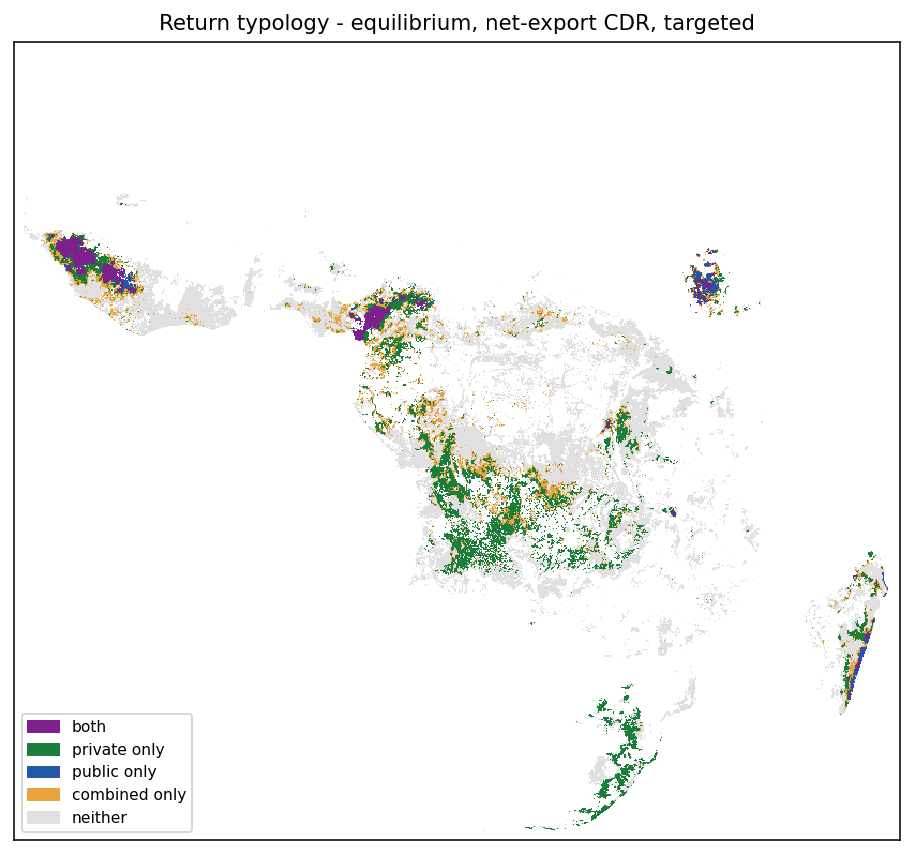
\includegraphics[width=0.72\textwidth]{env_typology_targeted_eqnx.png}
\caption{Return typology of SSA cropland in the equilibrium steady state with
net-export carbon accounting, targeted allocation. Purple = both private and
public returns independently sufficient (intersection); green = private-only;
blue = public-only; orange = combined-only (viable only when both streams are
stacked); grey = neither.}
\label{fig:typology}
\end{figure}

\begin{figure}[t]
\centering
\begin{subfigure}{0.33\textwidth}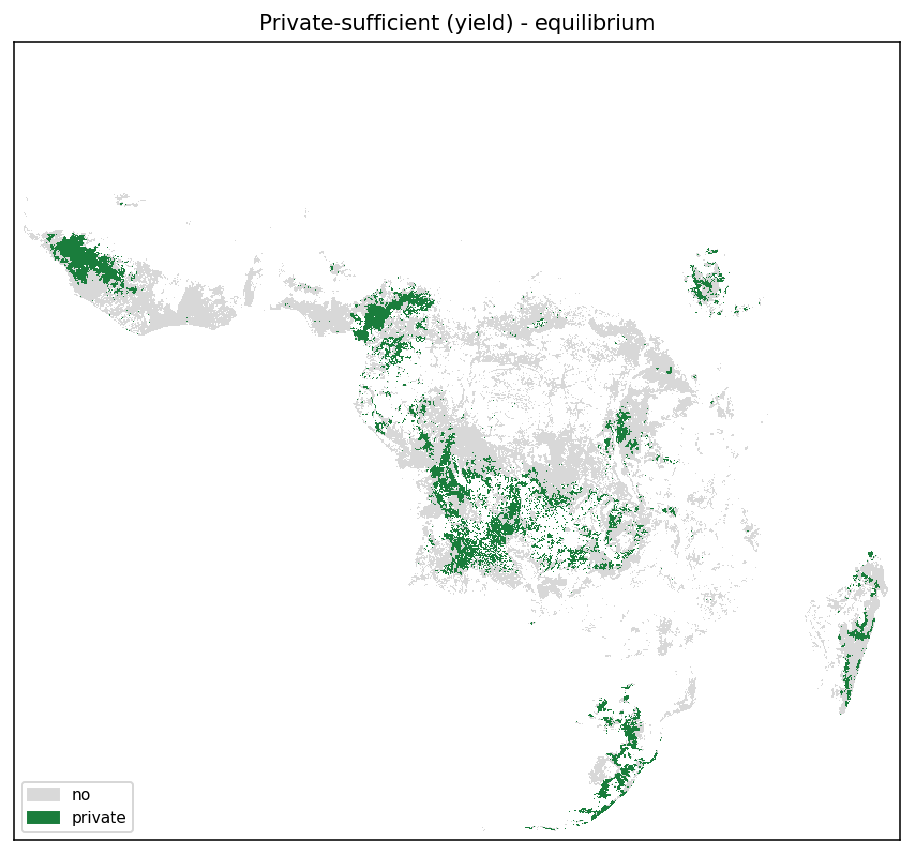
\includegraphics[width=\linewidth]{env_private_targeted_eqnx.png}\caption{Private}\end{subfigure}
\begin{subfigure}{0.33\textwidth}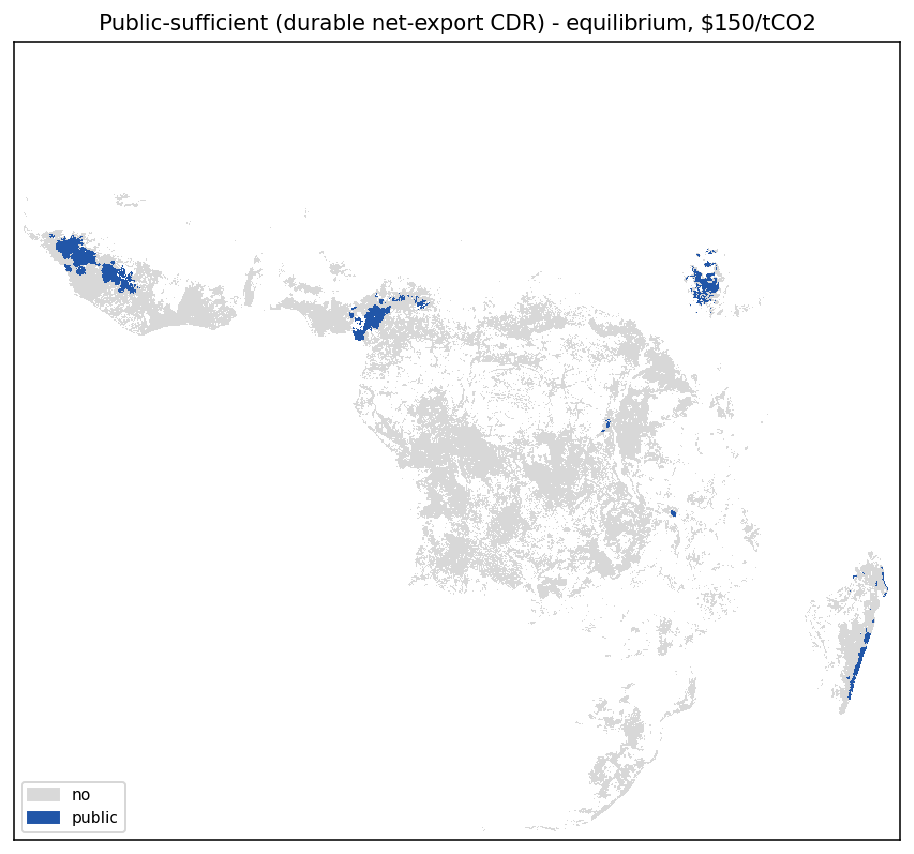
\includegraphics[width=\linewidth]{env_public_targeted_eqnx.png}\caption{Public}\end{subfigure}
\begin{subfigure}{0.33\textwidth}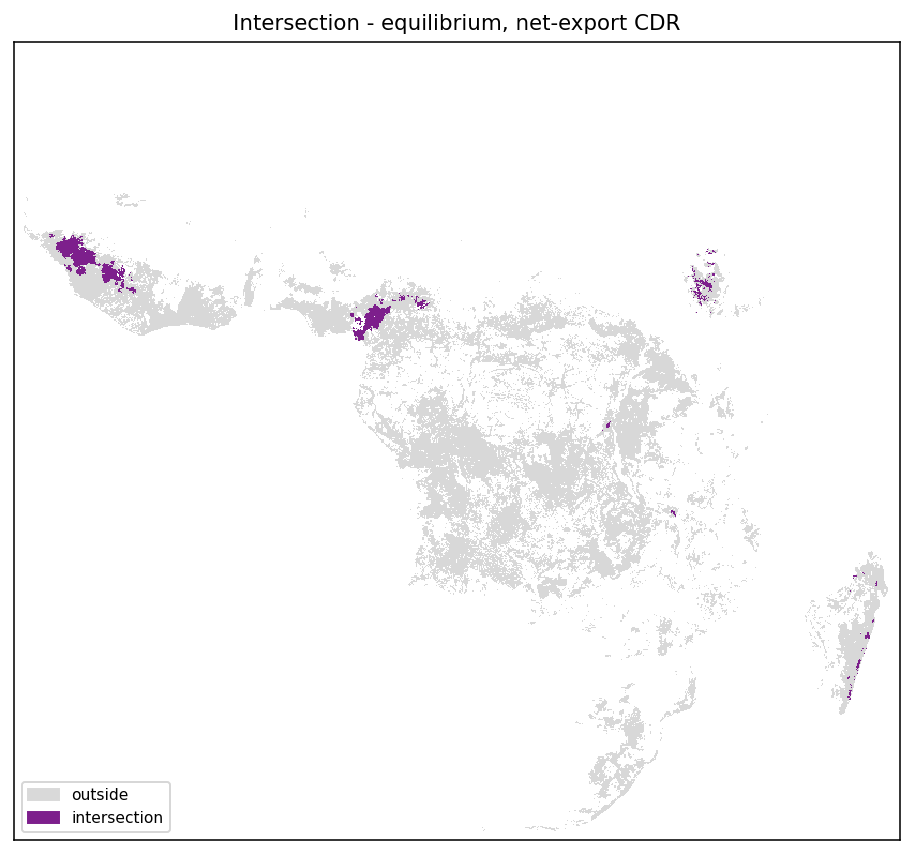
\includegraphics[width=\linewidth]{env_intersection_targeted_eqnx.png}\caption{Intersection}\end{subfigure}
\caption{The three envelopes mapped separately (equilibrium steady state,
net-export carbon accounting, targeted). Private: agronomic return exceeds
delivered cost. Public: durable net-export carbon revenue at \$150/\tco{}
exceeds delivered cost. Intersection: both hold.}
\label{fig:envelopes}
\end{figure}

\subsection{Durable carbon and the agronomy--carbon trade-off}\label{sec:durable}
The carbon figures above already net out the alkalinity consumed neutralizing
soil acidity (Section~\ref{sec:netexport}), and that deduction is first-order, not
cosmetic. At first application the standing acidity absorbs most of the weathered
alkalinity, so only about one-fifth of gross removal is durably exported
(targeted: 81~Mt gross $\to$ 19~Mt net; uniform: 101~$\to$~19~Mt). In the
equilibrium steady state, where the maintenance dose offsets only annual
re-acidification, most removal survives (targeted: 26~$\to$~19~Mt, 73\%; uniform:
101~$\to$~88~Mt, 87\%). Durable removal from ERW on acid soils is thus largely a
\emph{steady-state} phenomenon; the first application is, to first order, liming
with a small carbon tail -- which is why we evaluate the public case at
equilibrium.

The same accounting resolves how returns vary with soil pH. Both the yield
benefit and the gross weathering rate are largest on the most acidic soils, so a
naive model would place \emph{both} returns on the same low-pH land. Once the
acidity sink is deducted, the durable-carbon return shifts toward \emph{less}
acidic soils -- where less alkalinity is spent on neutralization and more
exports -- so the private and public returns become spatially complementary
(Figure~\ref{fig:schematic}). The corollary for deployment design: because the
lime-requirement dose is sized to the acidity demand, it is carbon-minimal;
maximizing durable removal requires applying \emph{beyond} agronomic need, so the
two objectives imply different optimal rates and the carbon payment must cover the
surplus rock that yields no extra harvest.

\begin{figure}[t]
\centering
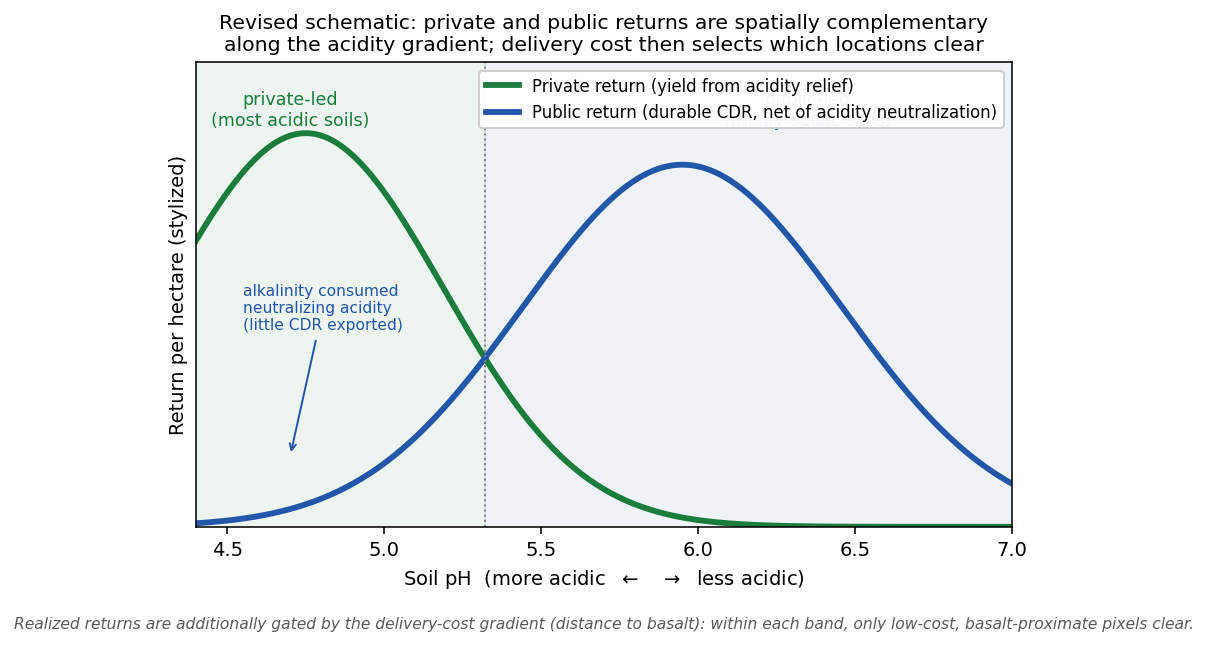
\includegraphics[width=0.78\textwidth]{revised_schematic_returns.png}
\caption{Private and public returns are spatially complementary along the soil-pH
gradient once durable (net-export) carbon is credited: private (yield) returns
peak on the most acidic soils; public returns peak on mildly acidic soils where
weathered alkalinity exports rather than neutralizing acidity. Realized returns
are then further selected by the delivery-cost gradient.}
\label{fig:schematic}
\end{figure}

Over-application also carries an agronomic cost that the base model omits: pushing
soil pH past the crop optimum reduces yield (Section~\ref{sec:overlime}). Charging
this over-liming penalty leaves the private return essentially unchanged at the
targeted dose but erodes it at high uniform rates, and it does so with sharply
increasing uncertainty (Figure~\ref{fig:overlime}). Centrally, the penalty reduces
the aggregate private return by about 7\% at the targeted dose, 6\% at uniform-10,
5\% at uniform-20, and 18\% at uniform-50; but the plausible range widens from a
tight 5--8\% at the agronomic dose to fully 3--99\% at uniform-50, depending on soil
buffering and realized reactivity. The direction is robust while the high-rate
magnitude is not: blanket high rates trade a bounded carbon gain for a large and
poorly-bounded yield risk, whereas the targeted dose avoids the exposure. This is
the third margin -- alongside rising cost and the acidity-sink deduction on CDR --
on which over-application is disfavored, and it completes the case for targeting
plus modest over-application rather than uniformly heavy rates.

\begin{figure}[t]
\centering
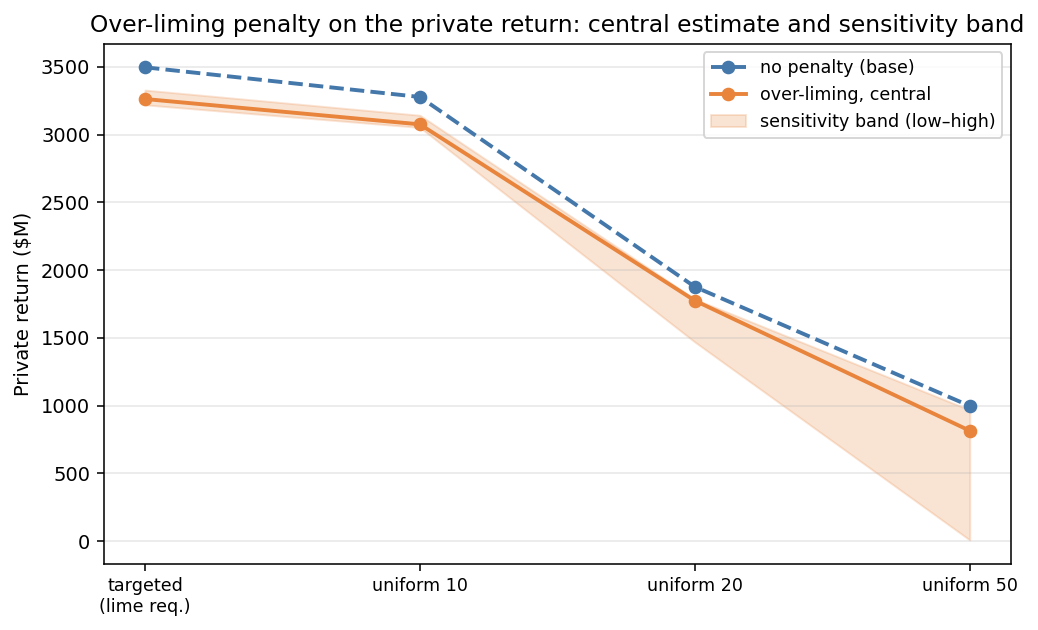
\includegraphics[width=0.72\textwidth]{overliming_sensitivity.png}
\caption{Over-liming penalty on the aggregate private return across the
application-rate ladder: no-penalty base, central estimate, and the sensitivity
band spanning soil-buffer and realized-reactivity assumptions. The band is tight at
the agronomic (targeted) dose and fans out at high uniform rates.}
\label{fig:overlime}
\end{figure}

\subsection{What binds the public (carbon) envelope}\label{sec:public}
Because ERW investment interest concentrates on the carbon case, we diagnose it
directly through the MAC test of equation~\eqref{eq:mac}, on durable net-export
removal. In the equilibrium steady state the area-weighted MAC has a median of
\textbf{\$446/\tco{}} (Figure~\ref{fig:mac}a), against a net credit price of only
\$130 (\$150 less \$20 MRV); only the cheapest fraction of land clears, which is
why the durable public envelope is 1.7~Mha. The contrast with first application
is stark: under net-export accounting the year-1/NPV median MAC rises to roughly
\$1{,}250/\tco{} and the carbon case all but disappears, because the standing
acidity must be paid down before any carbon exports -- again locating durable
removal in the steady state.

The durable public envelope of 1.7~Mha is 9.4\% of the treated cropland (1.1\% of
all SSA cropland), and its size is governed by the carbon price rather than by any
kinetic assumption: carbon-alone deployable area rises steeply as the price
climbs, from 2\% of treated cropland at \$100/\tco{} to 9\% at today's \$150,
28\% at \$350, and 50\% at \$500 (Table~\ref{tab:priceladder}). Two implications
follow. First, the physical removal potential is large but its \emph{economic}
viability under carbon revenue alone is price-limited: at present prices durable
CDR pays for its delivered cost on only about a tenth of the ERW-relevant
cropland. Second---and this is the crux of the argument---the fact that carbon
revenue rarely clears on its own is precisely why the private co-benefit matters.
Land that carbon alone cannot reach at \$150 becomes viable once the yield return
is stacked on top (the combined-only band, Section~\ref{sec:envelopes}); the
co-benefit is not a nicety but the mechanism that mobilizes voluntary carbon
finance across the region. And because the marginal abatement cost is the ratio of
delivered cost to \co{} removed per tonne, the two routes to broadening
carbon-alone viability are a higher realized CDR rate and cheaper delivery, both
of which lower it.

\begin{table}[t]
\centering
\caption{Carbon-alone deployability is price-conditional. Public-sufficient area
(durable net-export CDR revenue exceeds delivered cost) in the equilibrium steady
state, targeted allocation, across VCM carbon prices. Shares are of the 17.6~Mha
treated cropland; the all-cropland share (of 146~Mha) is shown for reference.}
\label{tab:priceladder}
\small
\begin{tabular}{rrrrr}
\toprule
VCM price (\$/\tco{}) & Public area (Mha) & \% treated & \% all cropland & Durable CDR (Mt) \\
\midrule
100 & 0.35 &  2.0 & 0.2 &  1.7 \\
150 & 1.65 &  9.4 & 1.1 &  4.8 \\
250 & 2.51 & 14.3 & 1.7 &  6.1 \\
350 & 4.84 & 27.6 & 3.3 & 11.0 \\
500 & 8.76 & 49.9 & 6.0 & 15.8 \\
\bottomrule
\end{tabular}
\end{table}

The binding factor is the realized \co{} removed per tonne of rock, $\delta_t$
(here on the order of 0.1 to 0.25 tonnes \co{} per tonne of rock), not the credit
price or logistics. Figure~\ref{fig:cdrrate} makes this quantitative (shown on the gross
NPV basis for comparability with the parameter grid): doubling $\delta_t$
raises the public envelope far more than a 33\% higher
carbon price or a 33\% delivered-cost reduction. $\delta_t$ is set by
the reactive fraction, grain size, the climate factor, and pedogenic-carbonate
loss -- the parameters that current process knowledge and MRV resolve least well.
The economic and the scientific frontier therefore coincide: the largest lever on
the carbon case is also the least-resolved quantity.

\begin{figure}[t]
\centering
\begin{subfigure}{0.49\textwidth}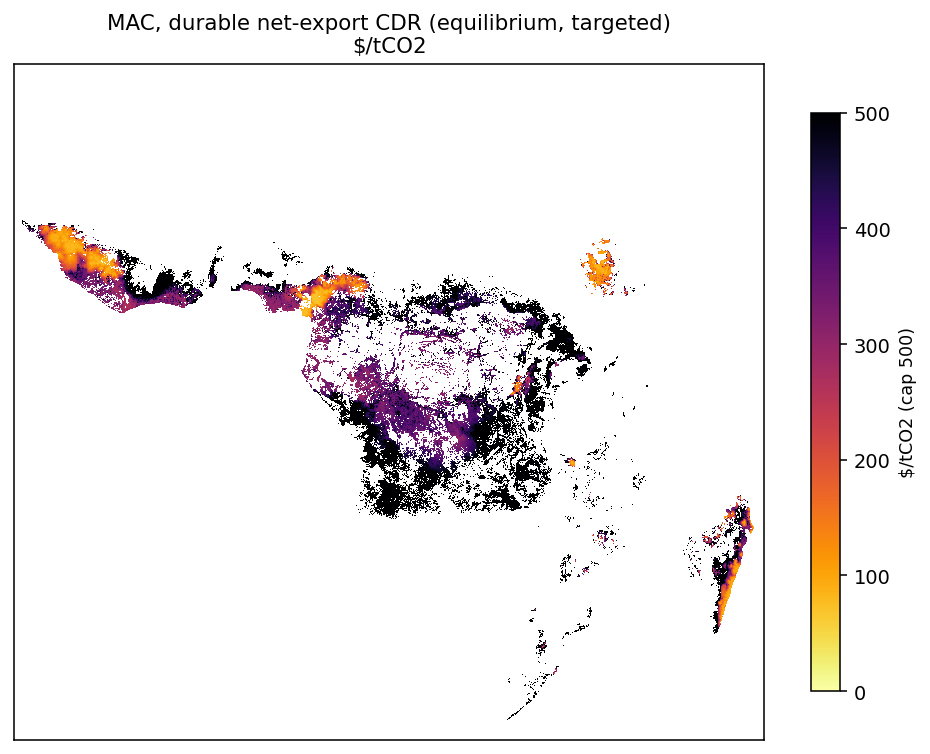
\includegraphics[width=\linewidth]{mac_targeted_eqnx.png}\caption{Marginal abatement cost (durable)}\end{subfigure}
\begin{subfigure}{0.49\textwidth}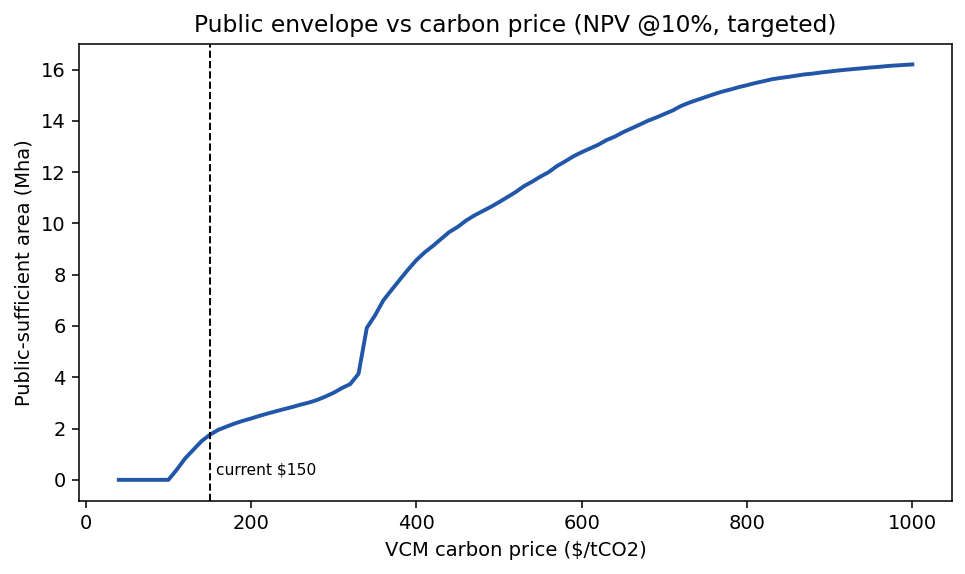
\includegraphics[width=\linewidth]{public_area_vs_price_npv.png}\caption{Public area vs.\ carbon price}\end{subfigure}
\caption{(a) Marginal abatement cost of durable net-export ERW-CDR (\$/\tco{},
capped at 500; equilibrium, targeted). (b) Public-sufficient area as a function of
the VCM carbon price (gross NPV accounting, an upper bound); the schedule is
steeply convex around current prices.}
\label{fig:mac}
\end{figure}

\begin{figure}[t]
\centering
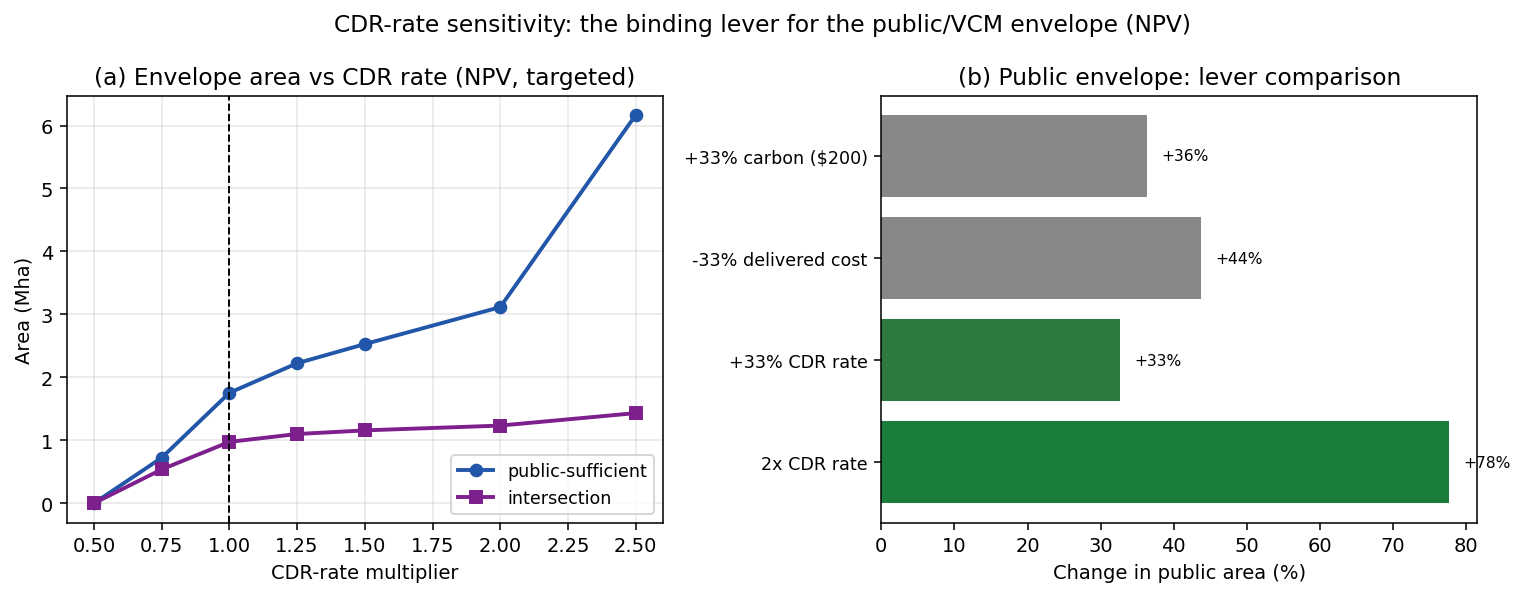
\includegraphics[width=0.95\textwidth]{cdr_rate_sensitivity_panel_npv.png}
\caption{The CDR rate is the binding lever for the public envelope.
(a) Public and intersection area versus the realized CDR-rate multiplier.
(b) Change in public-sufficient area under alternative levers: doubling the CDR
rate dominates plausible carbon-price or delivered-cost moves.}
\label{fig:cdrrate}
\end{figure}

\subsection{Cost-side levers: at-scale solar haulage}\label{sec:solar}
Transport is the largest single component of delivered cost (\(\sim\)56\% on
average, median \(\sim\)65\%) and is wholly variable in distance. We evaluate an
at-scale solar-electric haulage scenario that displaces the fuel/energy portion
of trucking cost. Grounding the energy share in trucking-cost data and the
diesel-to-solar-electric energy gap implies a feasible \(\sim\)25\% reduction in
the transport term (range 15--40\%), i.e.\ \(\sim\)14\% off average delivered
cost. Applied to the grid (NPV basis, for comparability with the sensitivity grid),
this widens the \emph{private} envelope materially
(2.0 to 2.6~Mha at $-$25\%, to 3.1~Mha at $-$40\%) but the public envelope only
slightly (1.8 to 1.9~Mha), confirming the asymmetry implied by
equation~\eqref{eq:mac}: cost reductions relax the private test directly but
relax the public test only to the extent the MAC falls below the credit price.
Carbon price and CDR rate move the public envelope; logistics cost moves the
private one. The two policy levers are thus complementary and target different
margins.

\subsection{Targeting and robustness}\label{sec:robust}
Repeating the envelope construction across the full parameter grid yields a
per-pixel robustness score (Figure~\ref{fig:core}). Under the NPV regime no
pixel survives the entire deliberately wide grid; the intersection is inherently
parameter-sensitive. A core-targeting tier (in the intersection under at least
half the grid) collapses to a small, high-confidence set concentrated in the
Cameroon highlands, while a broader candidate tier (at least one-third of the
grid) covers \(\sim\)0.8~Mha, \(\sim\)0.5~M farms, and \(\sim\)\$0.75~B of crop
value, extending into the Guinean and Ethiopian highlands -- areas where acidic
soils, a favorable weathering climate, basalt proximity, and adequate crop
prices coincide.

The carbon case behaves very differently across regimes once durable removal is
credited (Table~\ref{tab:regimes}). Under gross accounting the public envelope
looks broadly similar at first application and in steady state; under net-export
accounting it nearly vanishes at first application (NPV public
1.75~$\to$~0.14~Mha), because the standing acidity consumes the alkalinity, and
is restored only in the equilibrium steady state (2.23~$\to$~1.65~Mha), where the
maintenance dose offsets only annual re-acidification. The private envelope,
which does not depend on the carbon accounting, is stable across regimes. This
regime-dependence is precisely why we lead the carbon case on equilibrium.

\begin{table}[t]
\centering
\caption{Public envelope and total credited CDR (targeted), under gross versus
net-export accounting, at first application (NPV) and in steady state
(equilibrium). Net-export accounting collapses the first-application carbon case
and locates durable removal in the steady state.}
\label{tab:regimes}
\small
\begin{tabular}{lrrrr}
\toprule
Accounting & Public, NPV (Mha) & Public, equil.\ (Mha) & CDR, NPV (Mt) & CDR, equil.\ (Mt) \\
\midrule
Gross        & 1.75 & 2.23 & 81 & 26 \\
Net-export   & 0.14 & 1.65 & 19 & 19 \\
\bottomrule
\end{tabular}
\end{table}

\begin{figure}[t]
\centering
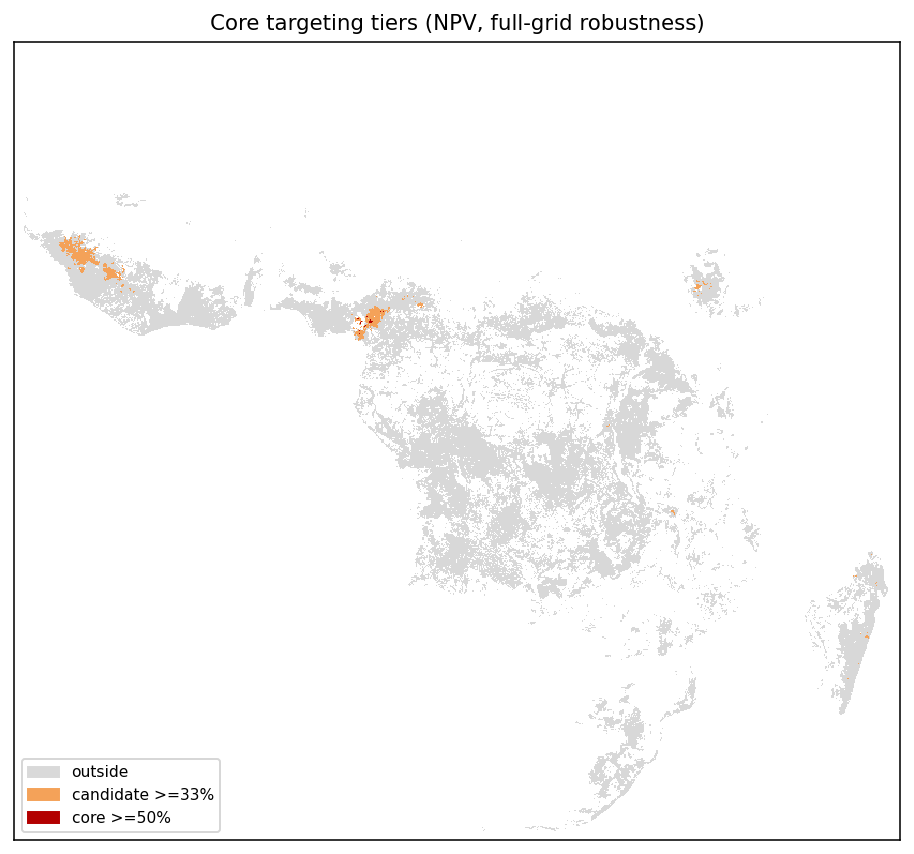
\includegraphics[width=0.72\textwidth]{core_priority_npv.png}
\caption{Core-targeting tiers under the NPV regime. Red = robust core
(intersection under $\geq$50\% of the parameter grid); orange = candidate tier
($\geq$33\%). The core concentrates where soil acidity, weathering climate,
basalt access, and crop value coincide.}
\label{fig:core}
\end{figure}

%=============================================================================
\section{Discussion}\label{sec:discuss}
% -- FULL PROSE ---------------------------------------------------------------
Three implications follow for the design of ERW programs and for the agricultural
economics of carbon-coupled practices more generally.

\paragraph{Carbon finance is the marginal, not the windfall, revenue.}
The dominance of the combined-only band means that on most ERW-viable SSA
cropland the agronomic return and the carbon return are each individually
insufficient to cover the upfront cost of crushed basalt, but their sum is not.
Voluntary carbon revenue is therefore best understood as the financing that
crosses the adoption threshold for a yield-enhancing practice that farmers would
otherwise forgo -- a framing closer to a cost-share or input subsidy than to a
pure carbon transaction. This both strengthens the additionality claim on that
land (the practice does not happen without the payment) and reframes the
distributional question: the credit buyer effectively subsidizes a private
yield gain, and program design must decide how that joint surplus is split
between buyer and farmer.

\paragraph{The carbon case is CDR-quantification risk, not price risk.}
Equation~\eqref{eq:mac} and Figure~\ref{fig:cdrrate} show that the public
envelope hinges on the realized removal per tonne of rock, the single largest
lever and the least-resolved scientific quantity. For investors this relocates
the central risk from the carbon market (price) to measurement, reporting, and
verification (quantity and durability). It also reframes MRV: the \$20/\tco{}
MRV cost is not merely a deduction but the mechanism that converts an uncertain
$\delta_t$ into a sellable, high-integrity tonne. Investment in cheaper, tighter
measurement raises the \emph{effective} CDR rate that can be monetized -- exactly
where the leverage lies.

\paragraph{Targeting and sequencing.} The robustness analysis points to a small
core geography that is attractive across a wide range of assumptions, and a
broader candidate tier for early deployment. Because cost-side and revenue-side
levers move different envelopes, an efficient program pairs logistics
investment (basalt siting, low-carbon haulage) where the private case is close,
with carbon-price or CDR-rate improvements where the public case is close.

\paragraph{Limitations.} The year-1 accounting is the most optimistic and the
NPV the most conservative; we report both. Farm counts use national average
holding sizes and are order-of-magnitude. The agronomic response and the climate
and pedogenic-carbonate terms remain empirical proxies; the CDR-rate sweep is our
stand-in for that structural uncertainty, and tighter field calibration is the
clear priority. We do not model tenure, who finances the upfront cost,
compaction or N\textsubscript{2}O effects, or country-level credit eligibility
(Article 6), each of which would refine the deployable geography.

%=============================================================================
\section{Conclusion}\label{sec:conclude}
% -- FULL PROSE ---------------------------------------------------------------
Enhanced Rock Weathering is unusual among carbon-removal options in paying a
farmer twice: once in yield and once in carbon. Mapping those two returns
separately across Sub-Saharan Africa shows that they rarely each suffice on their
own -- but that together they make a meaningful area of cropland profitable that
neither would alone. The policy object of interest is therefore the
\emph{combined-only} land, where voluntary carbon finance is the marginal
revenue that unlocks a yield-improving investment, and the binding technical
constraint is how much \co{} a tonne of rock verifiably removes. Treating ERW as
a coupled agronomic-and-carbon proposition, rather than as a pure CDR supply
curve, changes both where one would deploy it first and what one would invest in
to expand it.

%=============================================================================
\section*{Data and code availability}
All input layers are public; the analysis pipeline and the envelope/robustness
scripts (\texttt{erw-1}\,--\,\texttt{erw-11}) are in the project repository.

\section*{Acknowledgments}
This work was supported by the Bill \& Melinda Gates Foundation (BMGF) through
the Guiding Acid Soil Management Investments in Africa (GAIA) project (Grant
no.\ INV-029117), and the CGIAR Science Programs on Sustainable Farming and
Policy Innovations. We would like to thank all funders who supported this
research through their contributions to the CGIAR Trust Fund. The paper
benefited from useful comments and suggestions from \todo{XXX}.

\bibliographystyle{plainnat}
\bibliography{references}

\end{document}
